\chapter{宇宙学中的量子问题}
\label{chap:16}

\begin{chapteropening}
CMB 是最接近“整个宇宙作为光学实验”的观测对象，但它不是实验室里可以反复制备的量子光源。观测者得到的是一张带频率、偏振、角位置和噪声权重的天空图，再从图中估计角功率谱、相关函数、非高斯性和偏振旋转。量子语言出现在初始涨落、暴胀中的模式放大、两模压缩和退相干；数据语言则是 \(\mu{\rm K}\) 级温度涨落、\(E/B\) 偏振、\(C_\ell\)、\(f_{\rm NL}\)、张量标量比 \(r\) 和系统误差矩阵。COBE/FIRAS、COBE/DMR、WMAP/Planck、BICEP/Keck 和 CMB 偏振双折射分析给出了这些量的观测尺度 \citep{1967PhRvL..19.1199S,1990ApJ...354L..37M,1992ApJ...396L...1S,1994ApJ...420..439M,1996ApJ...473..576F,2009ApJ...707..916F,2020A&A...641A...1P,2020A&A...641A...5P,2020A&A...641A...6P,2020A&A...641A..10P,2021PhRvL.127o1301A}。
\end{chapteropening}

\section{CMB 首先是什么样的光场}

CMB 常被直接拿来谈暴胀量子涨落，但观测入口其实很朴素：望远镜先看到一个几乎完美黑体的微波天空，然后在这个平均背景上测 \(10^{-5}\) 量级的角向涨落和更弱的偏振结构。因此本章先从光场本身开始，再逐步退回到产生这些统计图样的早期量子模式。

平均 CMB 近似为温度
\[
  T_0 = 2.7255\pm0.0006\,{\rm K}
\]
的黑体。Planck 分布给出每个频率模式的平均光子占据数和比强度
\begin{equation}
  n_\nu
  =
  \frac{1}{\exp(h\nu/k_{\rm B}T_0)-1},
  \qquad
  I_\nu
  =
  \frac{2h\nu^3}{c^2}n_\nu .
  \label{eq:ch16-planck-spectrum}
\end{equation}
\begin{formulaexplain}[公式 (16.1) 解读]
\(n_\nu\) 是单个频率模式的平均光子数，\(I_\nu\) 是黑体比强度，\(T_0\) 是 CMB 平均温度。低频时 \(n_\nu\) 大，场更接近经典热光；高频时单模占据数下降，但总探测光子数仍由带宽和光束面积决定。
\end{formulaexplain}
\(\nu\) 用 Hz，\(I_\nu\) 的单位是 \({\rm erg\,s^{-1}\,cm^{-2}\,Hz^{-1}\,sr^{-1}}\)，CMB 文献常换成 \({\rm MJy\,sr^{-1}}\)。在 \(30\,{\rm GHz}\)，\(h\nu/k_{\rm B}T_0\simeq0.53\)，\(n_\nu\sim1.4\)，低频通道仍接近经典热场；在 \(150\,{\rm GHz}\)，\(n_\nu\simeq0.07\)，单模占据数已小于 1，但总光子数因望远镜带宽和角分辨元巨大而很高。黑体强度峰在 \(160\,{\rm GHz}\) 附近，这是 Planck HFI 和许多地面 CMB 实验选择 \(90/150/220\,{\rm GHz}\) 通道的物理背景。FIRAS 对黑体谱的精度把早期能量注入、谱畸变和非热辐射限制到极小水平，因此现代 CMB 宇宙学通常把平均谱当作已知背景，把信息放在角向涨落和偏振上 \citep{1994ApJ...420..439M,1996ApJ...473..576F,2009ApJ...707..916F}。

\begin{figure}[tbp]
\centering
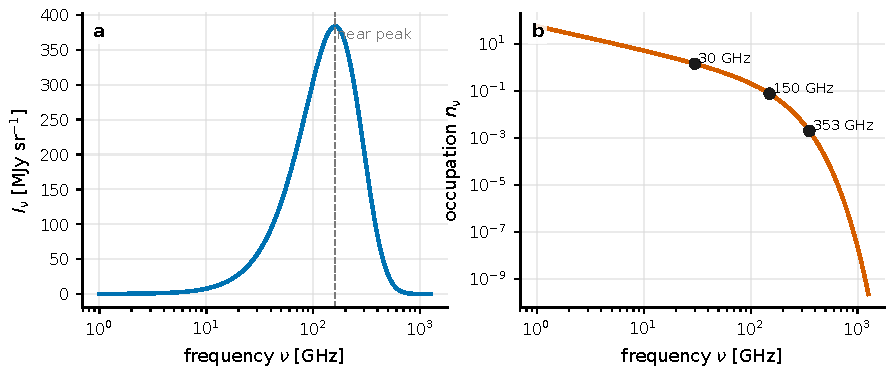
\includegraphics[width=0.94\linewidth]{figures/generated/chapter_16/ch16_cmb_blackbody.pdf}
\caption{CMB 的平均光场由黑体谱和模式占据数共同决定。左图把 \(T_0=2.7255\,{\rm K}\) 的 Planck 谱写成 \({\rm MJy\,sr^{-1}}\)，峰值在 \(160\,{\rm GHz}\) 附近。右图显示同一黑体在不同频率的单模平均光子数；低频通道占据数较高，高频通道逐渐进入 \(n_\nu<1\) 的量级。}
\label{fig:ch16-cmb-blackbody}
\end{figure}

角向涨落写成
\begin{equation}
  T(\hat{\bf n})
  =
  T_0\,[1+\Theta(\hat{\bf n})],
  \qquad
  \Theta(\hat{\bf n})
  =
  \sum_{\ell m}a_{\ell m}^{T}Y_{\ell m}(\hat{\bf n}).
  \label{eq:ch16-temperature-expansion}
\end{equation}
\begin{formulaexplain}[公式 (16.2) 解读]
\(\Theta(\hat{\bf n})\) 是无量纲温度涨落，\(a_{\ell m}^{T}\) 是球谐系数，\(Y_{\ell m}\) 是球谐函数。这条式子把一张天空图拆成角尺度模式：\(\ell\) 控制尺度，\(m\) 控制同一尺度上的方位自由度。
\end{formulaexplain}
\(\hat{\bf n}\) 是天空方向，\(a_{\ell m}^T\) 是无量纲温度涨落系数；实际图上常把 \(T_0\Theta\) 写成 \(\mu{\rm K}\)。COBE/DMR 首次在全天图上看到 \(\Delta T/T\sim10^{-5}\) 的结构，现代 Planck 地图把这个信号分解到 \(\ell\sim2500\) 量级。多极矩 \(\ell\) 与角尺度近似满足 \(\theta\simeq180^\circ/\ell\)：\(\ell\simeq2\) 对应半个天空，\(\ell\simeq200\) 对应一度角，\(\ell\simeq2000\) 对应几角分。各向同性高斯天空的角功率谱估计量为
\begin{equation}
  \widehat C_\ell^{TT}
  =
  \frac{1}{2\ell+1}
  \sum_{m=-\ell}^{\ell}
  |a_{\ell m}^{T}|^2,
  \qquad
  D_\ell^{TT}
  =
  \frac{\ell(\ell+1)}{2\pi}C_\ell^{TT}.
  \label{eq:ch16-cl-estimator}
\end{equation}
\begin{formulaexplain}[公式 (16.3) 解读]
\(\widehat C_\ell^{TT}\) 是温度角功率谱估计量，来自同一 \(\ell\) 上所有 \(m\) 模式的平均；\(D_\ell\) 是常用的重标度形式。这个平均就是 CMB 二点统计的核心压缩。
\end{formulaexplain}
\(C_\ell\) 的单位取决于 \(a_{\ell m}\) 是否乘了温度；若 \(a_{\ell m}\) 用 \(\mu{\rm K}\)，\(C_\ell\) 和 \(D_\ell\) 就是 \(\mu{\rm K}^2\)。\(D_\ell^{TT}\) 第一声学峰位于 \(\ell\simeq220\)，峰高约 \(5\times10^3\,\mu{\rm K}^2\)。这些峰来自光子-重子流体在复合前的声学振荡：重子密度改变压缩峰高度，暗物质密度改变引力势衰减，角直径距离把物理声学尺度投影成角尺度。Planck 2018 在六参数平直 \(\Lambda{\rm CDM}\) 中给出 \(\Omega_bh^2=0.0224\)、\(\Omega_ch^2=0.120\)、\(n_s=0.965\)、\(\tau=0.054\)、\(H_0=67.4\,{\rm km\,s^{-1}\,Mpc^{-1}}\)、\(\Omega_m=0.315\)、\(\sigma_8=0.811\) 的典型精度 \citep{1992ApJ...396L...1S,1996ApJ...469..437S,2020A&A...641A...5P,2020A&A...641A...6P,2021A&A...652C...4P}。

即使没有仪器噪声，全天也只给每个 \(\ell\) 的 \(2\ell+1\) 个 \(m\) 模式。高斯天空的 cosmic variance 为
\begin{equation}
  \frac{\sigma(C_\ell)}{C_\ell}
  =
  \sqrt{\frac{2}{(2\ell+1)f_{\rm sky}}},
  \label{eq:ch16-cosmic-variance}
\end{equation}
\begin{formulaexplain}[公式 (16.4) 解读]
\(\sigma(C_\ell)/C_\ell\) 是样本方差的相对误差，\(f_{\rm sky}\) 是有效天区比例。低 \(\ell\) 可用模式少，所以即使仪器完美，大角尺度也有无法消除的统计不确定性。
\end{formulaexplain}
\(f_{\rm sky}\) 是有效天空覆盖率。全天 \(\ell=2\) 的相对误差约 \(63\%\)，\(\ell=200\) 降到 \(7\%\)，\(\ell=2000\) 约 \(2.2\%\)；若银河面和强前景区被 mask，\(f_{\rm sky}<1\)，误差还会增大。因此低 \(\ell\) 异常、四极矩偏低或 hemispherical asymmetry 要放进有限模式数的协方差中，而不宜只凭单个点在图上的显眼程度判断。

\begin{figure}[tbp]
\centering
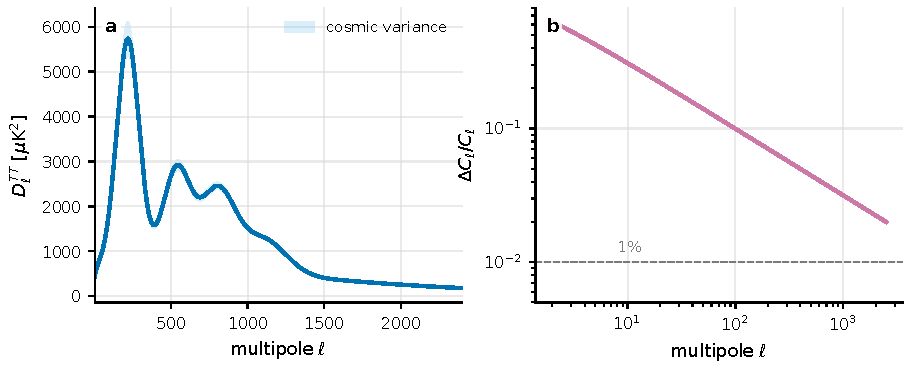
\includegraphics[width=0.94\linewidth]{figures/generated/chapter_16/ch16_cmb_power_spectrum.pdf}
\caption{角功率谱把天空涨落压缩到多极矩空间。左图是带声学峰和阻尼尾的标度图，蓝色阴影表示全天 cosmic variance 的量级；右图单独画出 \(\sqrt{2/(2\ell+1)}\)，显示大角尺度的误差由天空上可用模式数限制，望远镜灵敏度无法消除这部分方差。}
\label{fig:ch16-cmb-power}
\end{figure}

偏振图比温度图多两个 Stokes 参数。把 \(Q\) 和 \(U\) 组成 spin-2 场后，
\begin{equation}
  (Q\pm iU)(\hat{\bf n})
  =
  \sum_{\ell m}
  a_{\pm2,\ell m}\,{}_{\pm2}Y_{\ell m}(\hat{\bf n}),
  \qquad
  a_{\ell m}^{E}
  =
  -\frac{1}{2}(a_{2,\ell m}+a_{-2,\ell m}),
  \quad
  a_{\ell m}^{B}
  =
  \frac{i}{2}(a_{2,\ell m}-a_{-2,\ell m}).
  \label{eq:ch16-eb-definition}
\end{equation}
\begin{formulaexplain}[公式 (16.5) 解读]
\(Q\pm iU\) 是自旋 \(\pm2\) 的偏振场，\({}_{\pm2}Y_{\ell m}\) 是自旋球谐函数，\(a_{\ell m}^{E/B}\) 是 E/B 模系数。这个分解把局部偏振方向转换成全天天空上的标量型和旋量型图样。
\end{formulaexplain}
\(E\) 模在宇称变换下像标量，\(B\) 模像赝标量。标量密度涨落在线性阶主要产生 \(T\) 和 \(E\)，不直接产生原初 \(B\)；张量扰动、弱透镜、偏振角旋转、银河尘埃和同步辐射都能产生 \(B\)。因此，B 模检出需要和频率分离、delensing、角标定和 foreground model 一起解释，才能指向原初引力波。E/B 分解的全天天空形式来自 Zaldarriaga-Seljak 和 Kamionkowski-Kosowsky-Stebbins 的经典工作；后来的 BICEP/Keck 约束把这个数学分解变成了原初引力波搜索的主要观测通道 \citep{1997PhRvD..55.1830Z,1997PhRvL..78.2054S,1997PhRvL..78.2058K,2021PhRvL.127o1301A}。

\section{暴胀涨落为什么像两模压缩态}

上一节的 \(C_\ell\) 是天空上的统计量；暴胀理论要解释的是这些统计量为什么有近似高斯性、近似尺度不变性和固定声学相位。这里不能把 CMB 当成一束可反复制备的实验室光，而要把早期宇宙中的场模式当成时变谐振子。暴胀量子涨落通常不用单个光子的语言写，而是写成规范不变量的场模式。对标量曲率扰动 \(\mathcal R\)，定义 Mukhanov-Sasaki 变量
\begin{equation}
  v({\bf x},\eta)=z(\eta)\mathcal R({\bf x},\eta),
  \qquad
  z=\frac{a\dot\phi}{H},
  \label{eq:ch16-ms-variable}
\end{equation}
\begin{formulaexplain}[公式 (16.6) 解读]
\(v\) 是 Mukhanov-Sasaki 变量，\(\mathcal R\) 是曲率扰动，\(z=a\dot\phi/H\) 包含背景暴胀演化。用 \(v\) 写方程，可以把每个 Fourier 模看成一个时变频率的量子谐振子。
\end{formulaexplain}
\(\eta\) 是 conformal time，\(a\) 是尺度因子，\(\phi\) 是驱动暴胀的背景场，\(H=\dot a/a\)。在二阶作用量中，每个 Fourier 模近似是时变频率谐振子：
\begin{equation}
  v_k''+
  \left(k^2-\frac{z''}{z}\right)v_k
  =
  0 .
  \label{eq:ch16-ms-equation}
\end{equation}
\begin{formulaexplain}[公式 (16.7) 解读]
\(v_k\) 是共动波数 \(k\) 的模式函数，\(z''/z\) 是背景膨胀给出的有效势。亚视界时 \(k^2\) 主导，模式像真空振子；出视界后有效势主导，曲率扰动幅度被冻结。
\end{formulaexplain}
\(k\) 是共动波数，单位常用 \({\rm Mpc^{-1}}\)；撇号是对 \(\eta\) 求导。亚视界时 \(k\gg aH\)，方程近似 \(v_k''+k^2v_k=0\)，Bunch-Davies 真空取
\[
  v_k\simeq \frac{e^{-ik\eta}}{\sqrt{2k}}.
\]
当 \(k\simeq aH\) 穿出视界后，\(z''/z\) 项主导，增长解被冻结，衰减解迅速变小，\(\mathcal R_k=v_k/z\) 变成近似常数。这里的“冻结”指相位空间中一个象限被强烈压窄，最后只剩一个随机幅度控制后来的密度扰动；它并不表示模式完全停止演化 \citep{1988JETP...67.1297M,1990PhRvD..42.3413G,1996CQGra..13..377P}。

功率谱定义为
\begin{equation}
  \langle
  \mathcal R_{\bf k}\mathcal R_{{\bf k}'}
  \rangle
  =
  (2\pi)^3\delta^{(3)}({\bf k}+{\bf k}')
  \frac{2\pi^2}{k^3}
  \mathcal P_{\mathcal R}(k),
  \qquad
  \mathcal P_{\mathcal R}(k)
  =
  A_s
  \left(\frac{k}{k_*}\right)^{n_s-1}.
  \label{eq:ch16-primordial-spectrum}
\end{equation}
\begin{formulaexplain}[公式 (16.8) 解读]
\(\mathcal P_{\mathcal R}(k)\) 是无量纲原初曲率功率谱，\(A_s\) 是振幅，\(n_s\) 是谱指数，\(k_*\) 是 pivot。它把早期量子涨落的二点统计写成今天 CMB 拟合的核心参数。
\end{formulaexplain}
\(A_s\) 是无量纲振幅，Planck 常用 pivot \(k_*=0.05\,{\rm Mpc^{-1}}\)，并给出 \(\ln(10^{10}A_s)\simeq3.04\)，即 \(A_s\simeq2.1\times10^{-9}\)。\(n_s=1\) 是精确 scale-invariant；Planck 的 \(n_s\simeq0.965\) 表示红倾，长波模式略强。这个 \(10^{-9}\) 的原初曲率功率经过辐射转移函数、重子声学振荡、复合面厚度、透镜和平滑，投影成今天 \(\Delta T/T\sim10^{-5}\) 的天空涨落 \citep{2020A&A...641A...6P,2020A&A...641A..10P}。

在量子光学语言里，暴胀把 \({\bf k}\) 和 \(-{\bf k}\) 两个模式从真空演化成两模压缩态，
\begin{equation}
  |\psi\rangle
  =
  \prod_{\bf k}
  \exp\!\left[
    r_k e^{-2i\varphi_k}a_{\bf k}a_{-{\bf k}}
    -
    r_k e^{2i\varphi_k}a_{\bf k}^\dagger a_{-{\bf k}}^\dagger
  \right]
  |0\rangle .
  \label{eq:ch16-squeezed-state}
\end{equation}
\begin{formulaexplain}[公式 (16.9) 解读]
\(|\psi\rangle\) 是 \({\bf k}\) 与 \(-{\bf k}\) 成对的两模压缩态，\(r_k\) 是压缩强度，\(\varphi_k\) 是压缩角。暴胀的时变背景把真空涨落成对放大，并保留固定相位关系。
\end{formulaexplain}
\(r_k\) 是 squeezing parameter，\(\varphi_k\) 是 squeezing angle。平均占据数 \(N_k=\sinh^2r_k\)；超视界很久以后 \(r_k\) 很大，\(N_k\) 可指数增大。这里的“占据数”指早期场模式的量子激发数，和望远镜实际数到的 CMB 光子数不是同一个量。对经历 \(50-60\) 个 e-folds 后重新进入视界的模式，衰减象限已经极小，Wigner 函数像一条细长椭圆，后来的声学振荡继承了固定相位。这种固定相位解释了 CMB \(TT\)、\(TE\)、\(EE\) 谱中成串声学峰，而不是一团随机相位波纹 \citep{1990PhRvD..42.3413G,1996CQGra..13..377P,2006CQGra..23.2317P}。

\begin{figure}[tbp]
\centering
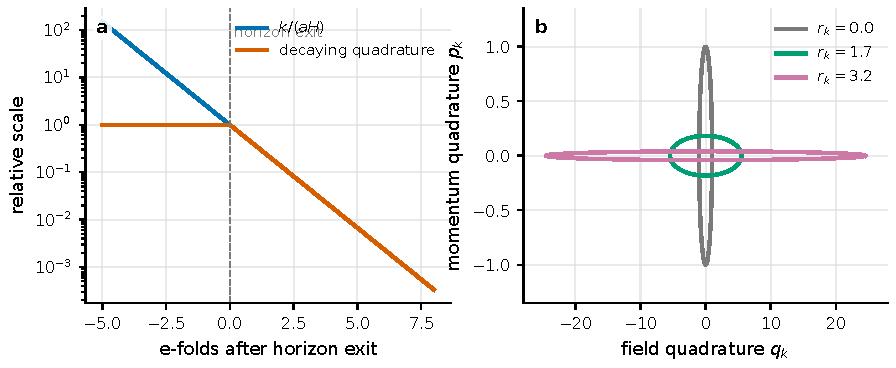
\includegraphics[width=0.94\linewidth]{figures/generated/chapter_16/ch16_squeezed_modes.pdf}
\caption{暴胀中的模式放大可以看成两模压缩。左图显示 \(k/(aH)\) 在穿出视界后指数下降，同时衰减象限被压小。右图画相空间椭圆：\(r_k\) 增大时，一个象限被拉长，另一个象限被压窄；观测到的是后来表现为经典随机幅度的长轴信息。}
\label{fig:ch16-squeezed}
\end{figure}

退相干把“纯压缩态”变成可用经典随机场描述的有效状态。这里的环境可以是未观测短波模式、张量/标量相互作用、复合前等离子体自由度、透镜势或数据处理中被 marginalize 掉的前景和仪器模式。写成密度矩阵时，观测变量 \(q_k\) 的有效约化矩阵近似为
\begin{equation}
  \rho_{\rm red}(q,q')
  =
  \rho_0(q,q')
  \exp\!\left[-\Gamma_k(q-q')^2\right],
  \label{eq:ch16-decoherence-density}
\end{equation}
\begin{formulaexplain}[公式 (16.10) 解读]
\(\rho_{\rm red}\) 是观测变量的约化密度矩阵，\(\rho_0\) 是未退相干形式，\(\Gamma_k\) 衡量环境抑制非对角项的强度。当 \(q\neq q'\) 的相干项被压低后，功率谱可用经典随机场语言计算。
\end{formulaexplain}
\(\Gamma_k\) 是退相干强度，单位取决于 \(q_k\) 的归一化。若 \(\Gamma_k(\Delta q)^2\gg1\)，不同幅度分支之间的干涉项被压低，功率谱和相关函数可按经典随机场计算。早期宇宙的“测量问题”仍有概念层面的争论；但对 \(C_\ell\)、\(B_\ell\) 和 lensing reconstruction 这些观测量而言，保留下来的相干相位信息不足以表现为实验室式 Bell 测试或可反复制备的非经典态 \citep{1996CQGra..13..377P,2006CQGra..23.2317P}。

\section{非高斯性和张量模式分别检验什么}

二点函数告诉我们“有多少涨落”；更高点函数和张量模式则问“这些涨落怎样产生”。非高斯性检验暴胀期间的相互作用和场内容，张量 B 模检验是否存在原初引力波背景。两者都很诱人，也都非常容易被有限模式数、透镜、尘埃和模板选择限制。

若 \(\mathcal R\) 是严格高斯场，所有信息都在二点函数中；三点函数和更高点函数为零。暴胀相互作用、非平凡声速、多场转移、激发初态或尖锐特征会产生非高斯性。三点函数写成
\begin{equation}
  \langle
  \mathcal R_{{\bf k}_1}
  \mathcal R_{{\bf k}_2}
  \mathcal R_{{\bf k}_3}
  \rangle
  =
  (2\pi)^3
  \delta^{(3)}({\bf k}_1+{\bf k}_2+{\bf k}_3)
  B_{\mathcal R}(k_1,k_2,k_3).
  \label{eq:ch16-bispectrum}
\end{equation}
\begin{formulaexplain}[公式 (16.11) 解读]
\(B_{\mathcal R}\) 是曲率扰动的 bispectrum，三个 \(k\) 必须由 delta 函数闭合成三角形。不同三角形形状对应不同早期宇宙相互作用，因此三点函数是非高斯性的主要语言。
\end{formulaexplain}
\(B_{\mathcal R}\) 的三个 \(k\) 构成一个三角形。local 型在 squeezed triangle 中最强，即 \(k_1\ll k_2\simeq k_3\)；equilateral 型在三边相等时最强；orthogonal 型是为区分不同相互作用而构造的近似正交模板。local ansatz 常写成
\begin{equation}
  \mathcal R({\bf x})
  =
  \mathcal R_g({\bf x})
  +
  \frac{3}{5}f_{\rm NL}^{\rm local}
  \left[
    \mathcal R_g^2({\bf x})
    -
    \langle\mathcal R_g^2\rangle
  \right],
  \label{eq:ch16-local-fnl}
\end{equation}
\begin{formulaexplain}[公式 (16.12) 解读]
\(\mathcal R_g\) 是高斯场，\(f_{\rm NL}^{\rm local}\) 是 local 型非高斯振幅。二次项让长波模式调制短波功率，因此 local 模板在 squeezed 构型中最敏感。
\end{formulaexplain}
\(\mathcal R_g\) 是高斯部分，\(f_{\rm NL}\) 无量纲。Planck 2018 的温度加偏振结果给出 \(f_{\rm NL}^{\rm local}=-0.9\pm5.1\)、\(f_{\rm NL}^{\rm equil}=-26\pm47\)、\(f_{\rm NL}^{\rm orth}=-38\pm24\) 的 \(68\%\) C.L. 约束，没有发现标准模板的显著非高斯性。单场慢滚暴胀的 squeezed-limit consistency relation 预言 local 非高斯很小，数量级与 \(1-n_s\) 相近；Maldacena 的三阶作用量计算是这个结论的标准来源 \citep{2003JHEP...05..013M,2020A&A...641A...9P,2020A&A...641A..10P}。

\begin{figure}[tbp]
\centering
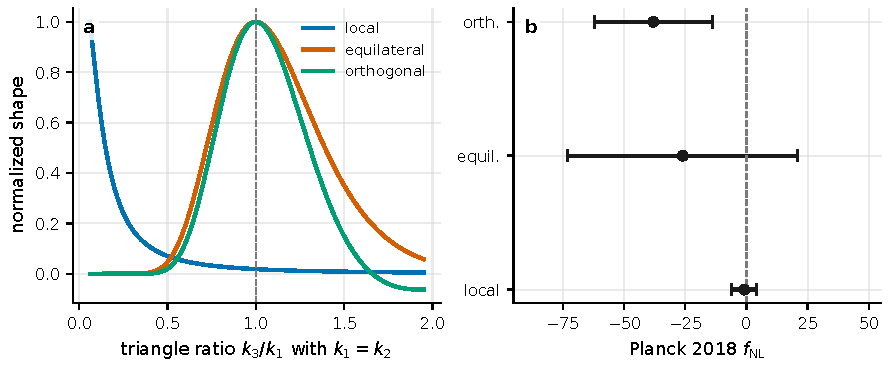
\includegraphics[width=0.94\linewidth]{figures/generated/chapter_16/ch16_non_gaussian_templates.pdf}
\caption{非高斯性由三角形构型和振幅共同决定。左图用 \(k_1=k_2\) 的切片比较 local、equilateral 和 orthogonal 模板的形状；local 型在 squeezed 极限增强，equilateral 型在三边接近相等时最大。右图给出 Planck 2018 对三个常用 \(f_{\rm NL}\) 参数的代表性约束，误差条均与零相容。}
\label{fig:ch16-nongaussian}
\end{figure}

张量扰动是量子引力背景最直接的 CMB 目标。定义
\begin{equation}
  r(k_*)=
  \frac{\mathcal P_t(k_*)}{\mathcal P_{\mathcal R}(k_*)},
  \qquad
  \mathcal P_t(k)
  =
  A_t\left(\frac{k}{k_*}\right)^{n_t}.
  \label{eq:ch16-tensor-r}
\end{equation}
\begin{formulaexplain}[公式 (16.13) 解读]
\(r\) 是张量功率谱和标量曲率功率谱在 pivot \(k_*\) 处的比值，\(\mathcal P_t\) 用振幅 \(A_t\) 和 tilt \(n_t\) 描述。它把原初引力波背景压缩成 CMB B 模搜索最常引用的参数。
\end{formulaexplain}
\(r\) 无量纲，pivot 常取 \(0.002\) 或 \(0.05\,{\rm Mpc^{-1}}\)，不同下标不能混用。单场慢滚给出近似 consistency relation \(n_t\simeq-r/8\)。若把 \(r\) 转成暴胀能标，
\begin{equation}
  V_*^{1/4}
  \simeq
  1.06\times10^{16}\,{\rm GeV}
  \left(\frac{r}{0.01}\right)^{1/4},
  \label{eq:ch16-inflation-scale}
\end{equation}
\begin{formulaexplain}[公式 (16.14) 解读]
\(V_*^{1/4}\) 是暴胀能标，\(r\) 是张量标量比。因为四次方根关系，即使 \(r\) 的上限大幅改善，能标约束也只缓慢收紧。
\end{formulaexplain}
这里假设爱因斯坦引力、标准慢滚和单一能量标尺。Planck 2018 单独给出 \(r_{0.002}<0.10\) 的 \(95\%\) C.L. 上限；结合 BK15 B 模偏振得到 \(r_{0.002}<0.056\)，对应 \(V_*^{1/4}<1.6\times10^{16}\,{\rm GeV}\)。BICEP/Keck 2018 season 与 Planck、WMAP 联合分析给出 \(r_{0.05}<0.036\) 的 \(95\%\) C.L. 上限，并指出无 lensing 或无尘埃的理想模拟会显著降低 \(\sigma(r)\)；目前限制同时受 lensing B 模和银河尘埃影响 \citep{2020A&A...641A..10P,2021PhRvL.127o1301A,2019JCAP...02..056A}。

\begin{figure}[tbp]
\centering
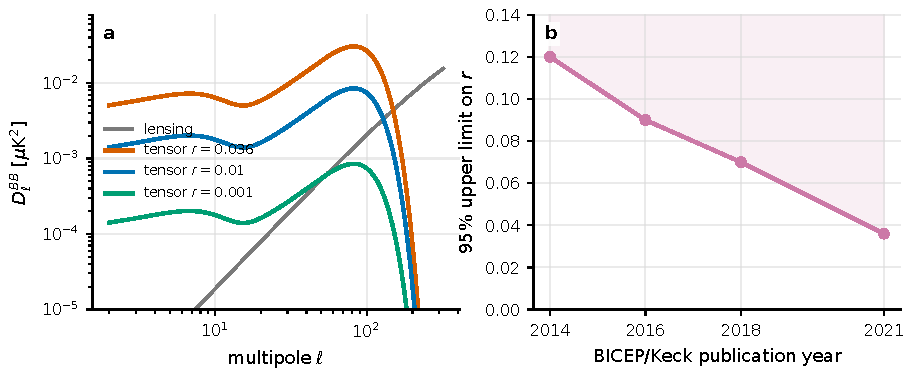
\includegraphics[width=0.94\linewidth]{figures/generated/chapter_16/ch16_bmode_constraints.pdf}
\caption{张量模式主要通过 B 模偏振受限。左图比较透镜 B 模和不同 \(r\) 的原初 tensor B 模标度；\(\ell\sim80\) 的 recombination bump 是地面实验的主战场，低 \(\ell\) reionization bump 需要大天区控制。右图显示 BICEP/Keck 系列联合约束从 \(r<0.12\) 改进到 \(r_{0.05}<0.036\) 的量级。}
\label{fig:ch16-bmode}
\end{figure}

\section{CMB 偏振双折射怎样区分宇宙角和仪器角}

第 \ref{chap:15} 章已经把轴子样场造成的偏振旋转写成 Stokes 量和 \(E/B\) 模混合，见式 \eqref{eq:ch15-qu-rotation} 和式 \eqref{eq:ch15-cmb-eb-tb}。放到 CMB 里，它首先变成一个校准问题：天空真的转过一个角，和仪器偏振角整体错一个角，在 \(EB/TB\) 统计中几乎同向。在 CMB 分析里，观测任务是把一个很小的全局角 \(\beta\) 从探测器角标定、银河尘埃、同步辐射和 map-making residual 中分出来。\(\beta\) 用弧度代入三角函数；\(0.35^\circ=6.1\times10^{-3}\,{\rm rad}\)，因此在小角度极限 \(EB/(EE-BB)\simeq2\beta\simeq1.2\%\)。这个百分之一信号足够大，可以在 Planck 级全天数据里留下统计迹象；也足够小，任何绝对偏振角标定、尘埃 EB、bandpass mismatch 或 beam leakage 都可能伪装它 \citep{2020PhRvL.125v1301M,2022PhRvD.106f3503E,2022PhRvL.128i1302D,2022NatRP...4..452K}。

\begin{figure}[tbp]
\centering
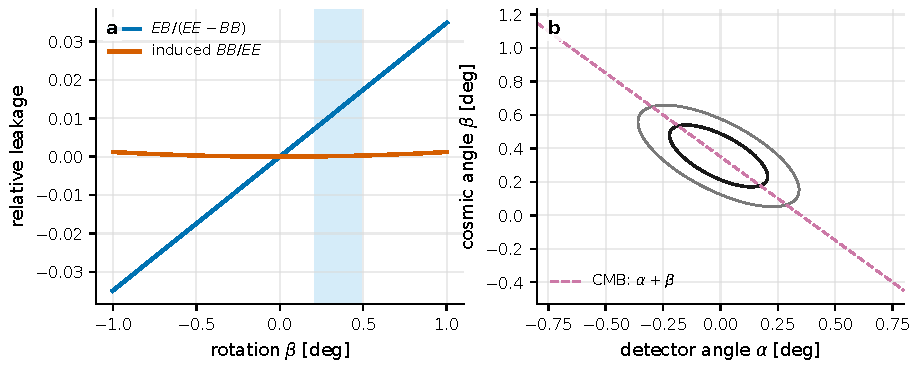
\includegraphics[width=0.94\linewidth]{figures/generated/chapter_16/ch16_birefringence_eb.pdf}
\caption{CMB 双折射把偏振角误差和宇宙学信号放在同一个平面里。左图显示 \(\beta\) 对 \(EB\) 和诱导 \(BB\) 的小角度泄漏；蓝色阴影标出 \(\beta=0.35\pm0.14^\circ\) 的量级。右图显示 detector angle \(\alpha\) 和 cosmic angle \(\beta\) 的退化方向：只用 CMB 时主要测到 \(\alpha+\beta\)，加入前景频率和多极矩信息才可能分离两者。}
\label{fig:ch16-birefringence}
\end{figure}

Minami 和 Komatsu 的 Planck 2018 分析利用 CMB 与银河前景偏振的不同频率依赖，同时估计 detector miscalibration \(\alpha_\nu\) 和 cosmic birefringence \(\beta\)，得到 \(\beta=0.35\pm0.14^\circ\)，并把地面角标定 \(0.28^\circ\) 的系统误差从最终误差中分离出去。后续 WMAP+Planck PR4 分析在 \(23-353\,{\rm GHz}\) 范围内加入 LFI/HFI 和 dust EB 模型，给出近全天 \(\beta=0.342^{+0.094}_{-0.091}{}^\circ\)，显著性约 \(3.6\sigma\)，但 polarized dust 的 intrinsic \(EB\)、低频 synchrotron EB 和独立角标定仍是主要限制。把这个信号解释成轴子样场时，旋转角来自
\begin{equation}
  \beta
  =
  \frac{1}{2}g_{\phi\gamma}
  [\phi(t_0)-\phi(t_{\rm LSS})],
  \label{eq:ch16-axion-birefringence}
\end{equation}
\begin{formulaexplain}[公式 (16.15) 解读]
\(\beta\) 是 CMB 偏振全局旋转角，\(g_{\phi\gamma}\) 是场-光子耦合，括号内是今天和最后散射面之间的场值差。若旋转来自轴子样传播效应，它应近似无频率依赖。
\end{formulaexplain}
\(g_{\phi\gamma}\) 的单位是 \({\rm GeV^{-1}}\)，\(\phi\) 是从最后散射面到今天的有效场值差。这个式子假设旋转近似各向同性、频率无关，并且源自传播过程而非发射面本征 \(EB\)。若 \(\beta(\nu)\propto\nu^{-2}\)，更像 Faraday 旋转；若 \(\beta\) 随天区、红移或时间变化，则需要从单个全局角推广到方向依赖或时间依赖的相关函数 \citep{2020PhRvL.125v1301M,2022PhRvL.128i1302D,2022NatRP...4..452K}。

\section{CMB 怎样与光学量子天文学对接}

CMB 和前几章的光学量子天文学共享“相关函数”语言，但观测含义不同。前几章更多处理可重复观测的源、可调的频带和可设计的探测链；CMB 则只有一片天空、一个初始条件和一套必须被充分建模的前景。这个差别决定了两边的“量子”不能简单互相替换。

实验室或恒星 HBT 中常用
\[
  g^{(2)}(\tau)
  =
  \frac{\langle I(t)I(t+\tau)\rangle}{\langle I\rangle^2}
\]
直接描述探测器时间序列中的强度涨落；CMB 的基本二点函数是天空球面上的
\begin{equation}
  \langle
  X_{\ell m}Y_{\ell' m'}^*
  \rangle
  =
  C_\ell^{XY}\delta_{\ell\ell'}\delta_{mm'},
  \qquad
  X,Y\in\{T,E,B,\phi_{\rm lens}\}.
  \label{eq:ch16-cmb-correlator}
\end{equation}
\begin{formulaexplain}[公式 (16.16) 解读]
\(C_\ell^{XY}\) 是两个天空场 \(X,Y\) 的角功率谱，Kronecker delta 表示在各向同性天空中不同 \(\ell,m\) 模式不相关。它是 CMB 版的二点相关函数语言。
\end{formulaexplain}
\(g^{(2)}\) 的时间延迟和带宽由仪器可主动选择；\(C_\ell\) 的模式数由宇宙给定，观测者只能改变 sky mask、频率组合、beam、noise weighting 和前景模型。CMB 无法像实验室系统那样调制源、重复制备初态或改变量子态；它提供的是早期场模式统计信息在 \(T/E/B\)、lensing 和 higher-order correlations 中的投影。

在 map-level 分析中，频率图、偏振图和外部 tracer 都进入同一个数据向量 \({\bf d}\)：
\begin{equation}
  {\bf d}
  =
  {\bf P}
  [
    {\bf s}_{\rm CMB}({\boldsymbol\theta})
    +
    {\bf s}_{\rm fg}({\boldsymbol\eta})
  ]
  +
  {\bf n},
  \qquad
  -2\ln\mathcal L
  =
  ({\bf d}-{\bf m})^{\mathsf T}
  C^{-1}
  ({\bf d}-{\bf m})
  +
  \ln\det C .
  \label{eq:ch16-cmb-likelihood}
\end{equation}
\begin{formulaexplain}[公式 (16.17) 解读]
\({\bf d}\) 是地图级数据向量，\({\bf P}\) 是观测和制图算子，\({\bf s}_{\rm CMB}\) 与 \({\bf s}_{\rm fg}\) 是宇宙信号和前景，\({\bf n}\) 是噪声。似然把模型残差和总协方差 \(C\) 放在一起，是从天空图推断宇宙学参数的工作形式。
\end{formulaexplain}
\({\bf P}\) 包含 beam、mask、scan strategy、bandpass 和 map-making；\({\boldsymbol\theta}\) 是宇宙学参数，例如 \(A_s,n_s,\Omega_bh^2,\Omega_ch^2,\tau,r,\beta\)；\({\boldsymbol\eta}\) 是前景参数，例如尘埃温度、谱指数、同步辐射谱指数和空间去相关；\(C\) 包括仪器噪声、样本方差、前景剩余和校准不确定性。Planck、Simons Observatory 和未来 CMB-S4/LiteBIRD 类实验的差别主要体现在 \({\bf P}\)、\(C\)、频率覆盖、角分辨率和可控系统误差上 \citep{2016A&A...594A..13P,2016A&A...594A..20P,2017MNRAS.472.1195C,2019JCAP...02..056A,2020A&A...641A...6P}。

读 CMB 文献时，单位和 pivot 最容易混淆。\(T_0\) 是 K，涨落图常用 \(\mu{\rm K}\)，而原初 \(\mathcal P_{\mathcal R}\) 是无量纲；\(A_s\sim2.1\times10^{-9}\) 不能直接和 \(D_\ell^{TT}\sim5000\,\mu{\rm K}^2\) 相比，中间有辐射转移函数。\(k\) 是 \({\rm Mpc^{-1}}\)，\(\ell\) 是角向模式数，粗略关系是 \(\ell\simeq kD_A(z_*)\)，其中 \(D_A(z_*)\) 是最后散射面的共动角直径距离。\(r\) 的 pivot 不统一，\(r_{0.002}\) 和 \(r_{0.05}\) 不是同一个数，尤其当 \(n_t\) 被放开时不能直接混用。量子网络望远镜会把讨论带回可控实验系统；CMB 则给出相反极限：初态不可重做，光路不可重置，但天空相关函数记录了早期宇宙量子涨落留下的统计痕迹。

